%%%%%%%%%%%%%%%%%%%%%%%%%%%%%%%%%%%%%%%%%%%%%%%%%%%%%%%%%%%%%%%%%%%%%%
% Report on LEGO Control Laboratory Manual.tex
% Last updated on 24th June 2014
% by S.R.Manikandasriram
%
% Template Source: http://www.howtotex.com
%
% Feel free to distribute this example, but please keep the referral
% to howtotex.com
% Date: March 2011 
% 
%%%%%%%%%%%%%%%%%%%%%%%%%%%%%%%%%%%%%%%%%%%%%%%%%%%%%%%%%%%%%%%%%%%%%%
% Edit the title below to update the display in My Documents
\title{LEGO based Control System Laboratory - An Analysis}
%
%%% Preamble
\documentclass[paper=a4, fontsize=11pt]{scrartcl}
\usepackage[T1]{fontenc}
\usepackage{lmodern}

\usepackage[english]{babel}          % English language/hyphenation
\usepackage[protrusion=true,expansion=true]{microtype}  
\usepackage{amsmath,amsfonts,amsthm} % Math packages
\usepackage[pdftex]{graphicx}   
\usepackage{url}


%%% Custom sectioning
\usepackage{sectsty}
\allsectionsfont{\centering \normalfont\scshape}


%%% Custom headers/footers (fancyhdr package)
\usepackage{fancyhdr}
\pagestyle{fancyplain}
\fancyhead{}                                            % No page header
\fancyfoot[L]{}                                         % Empty 
\fancyfoot[C]{}                                         % Empty
\fancyfoot[R]{\thepage}                                 % Pagenumbering
\renewcommand{\headrulewidth}{0pt}                      % Remove header underlines
\renewcommand{\footrulewidth}{0pt}                      % Remove footer underlines
\setlength{\headheight}{13.6pt}


%%% Equation and float numbering
\numberwithin{equation}{section}        % Equationnumbering: section.eq#
\numberwithin{figure}{section}          % Figurenumbering: section.fig#
\numberwithin{table}{section}           % Tablenumbering: section.tab#


%%% Maketitle metadata
\newcommand{\horrule}[1]{\rule{\linewidth}{#1}}     % Horizontal rule

\title{
        %\vspace{-1in}  
        \usefont{OT1}{bch}{b}{n}
        \normalfont \normalsize \textsc{Indian Institute of Technology Madras} \\ [25pt]
        \horrule{0.5pt} \\[0.4cm]
        \huge LEGO Control Systems Laboratory Manual \\
        \horrule{2pt} \\[0.5cm]
}
\author{
        \normalfont                                 \normalsize
        S.R.Manikandasriram\\[-3pt]      \normalsize
        \today
}
\date{}


%%% Begin document
\begin{document}
\maketitle

\begin{abstract}
This report analyses the scope of using the LEGO Mindstorms NXT Kit as a platform for teaching Control Engineering concepts for both Undergraduate and Graduate students. A set of simple experiments using only a LEGO DC Motor and the ``NXT Intelligent Brick'' have been analysed. The experiments cover the introductory concepts in Control Engineering like Transfer Function, PID Control, System Identification and Bode Plots and is thus ideal for an Undergraduate Laboratory course on Control Systems. The later half of the report deals with building a 2-wheel Self-balancing Robot using LEGO Mindstorms kits and a HiTechnic Gyro sensor. The mathematical model of the \emph{Segway} type robot is explained in detail and a Servo PID control for stabilising the \emph{Inverted Pendulum} is studied. This would be ideal as a Course Project for first year Masters students.
\end{abstract}

\pagebreak

\section*{Acknowledgement}

There is a number of publications on the use of LEGO NXT kits as an educational platform for undergraduate engineering students which provided valuable insights for our analysis. In particular, the first set of experiments discussed in this report is an extension of the paper \emph{A LEGO based Undergraduate Control Systems Laboratory} by Sabiha~A~Wadoo and Rahul~Jain. Also, the 2-wheel self-balancing robot project discussed in this report is an adaptation of the paper \emph{NXTway-GS Model based design} by Y.Yamamoto in 2008.

\pagebreak

\section{Introduction}
The use of LEGO Mindstorms series of kits as a platform for education has received widespread acceptance since the release of Mindstorms Robotics Invention System in 2000. The LEGO Mindstorms NXT kit is relatively cheap, robust, customizable, reprogrammable and induces enthusiasm and creativity in students. The official software for LEGO NXT is a NI LabView based programming language called NXT-G. However, enthusiasts have extended the software and hardware in various ways to make the LEGO NXT kits as a favourable Rapid prototyping platform for academic and research activities. In this report, we analyse the scope of using LEGO NXT kits for teaching Control Engineering. 
\\~\\
A para on the hardware specs and the programming environments.
\\~\\
A para on the other work done on this field
\\~\\
A para on the layout of this report
\section{Analysing the LEGO DC Motor}
The first half of the report explains relatively simple control experiments for analysing a DC Motor system. The analysis is divided into 4 parts - 1. Observing the in-built PID Controller, 2. Writing custom PID controller to meet design requirements, 3. Determining the Transfer Function of the DC Motor and 4. Designing PID controller using the derived Transfer Function. In order to avoid students from having to get used to a new programming language, ROBOTC - a C-like programming language developed by Carnegie Mellon University's Robotics Academy - will be used as software for this section. 

\subsection{Observe PID Controller in action}
In this first experiment, the students observe the functioning of the in-built PID Controller available in ROBOTC. The system under analysis is comprised of an \emph{Interactive Servo motor} which is controlled by Pulse Width Modulation by the NXT Intelligent Brick. The feedback is provided by the \emph{rotary encoder} present inside the \emph{Interactive Servo motor} which gives 360 counts per single revolution of the motor shaft. The block diagram for the PID controller is shown in~Figure~\ref{fig:block_diagram}. Using the feedback from the encoders, the ``\emph{NXT Intelligent Brick}'' calculates the angular position of the motor (with 1 degree accuracy) and also the instantaneous speed of the motor. The formula used for speed calculation is
\begin{equation}
speed = \frac{\Delta\theta}{\Delta{}t} \text{degrees/sec}
\end{equation}
\begin{figure}[!hbp]
	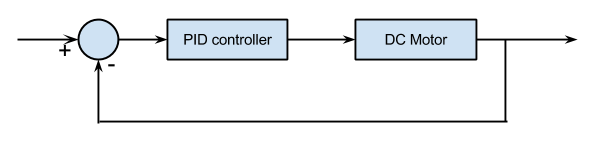
\includegraphics[width=0.5\textwidth]{block_diagram}
	\caption{Block Diagram of the in-built closed loop PID Controller}
	\label{fig:block_diagram}
\end{figure}

\begin{figure}[!hbp]
	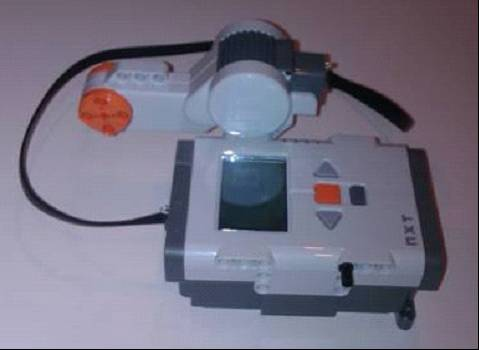
\includegraphics[width=0.5\textwidth]{setup}
	\caption{Experimental setup for observing in-built PID Controller}
	\label{fig:setup}
\end{figure}

The LEGO motors are assigned a power rating between $-100$ and $100$ with a negative value denoting reverse direction. Under ideal conditions, the maximum speed of the LEGO motors is $1000$ degrees per second when the power rating is set at $100\%$. But this value drops with decrease in battery voltage and increase in motor load. 

To enable PID Speed Control and set the maximum regulated speed, the following commands were used
\begin{verbatim}
nMotorPIDSpeedCtrl[motorB] = mtrSpeedReg;
nMaxRegulatedSpeedNxt = 750;
\end{verbatim}
The in-built PID controller provides consistent speed by continuously adjusting the raw power sent to the motor.

The LEGO NXT has a \emph{Datalog} feature which allows sensor data and status information to be stored in memory as \verb|(Key,Value)| pairs, which can later be exported to a PC for post-processing. In this experiment, the encoder counts and Motor PWM level are logged every $\Delta{}t  \text{ms}$. The ROBOTC code for this experiment is given below as the motive of this experiment is to get the students acquainted with the software and hardware interfaces. 
\begin{verbatim}
task main()
{
  nMaxRegulatedSpeedNxt = 500;
  // Reset the Motor Encoder
  nMotorEncoder[motorB] = 0;
  nMotorPIDSpeedCtrl[motorB] = mtrSpeedReg;

  int motorRAWpower, motorDegrees;
  motor[motorB] = 50;    // 50/100
  time1[T1] = 0;         // Timer

  // Allocate memory for datalog
  nDatalogSize = 1600;

  while (time1[T1] < 10000) {
    motorDegrees = nMotorEncoder[motorB];
    motorRAWpower = motorPWMLevel[motorB];     
    // store value to Datalog
    AddToDatalog(1,motorPIDdegrees);
    AddToDatalog(2,motorPIDpower);
    wait1Msec(50);
  }
  motor[motorB] = 0;   // Stop the motors
  SaveNxtDatalog();
}
\end{verbatim}

In order to observe the PID control action, the students are asked to run the above program and apply friction on the motor. The in-built PID controller will then step in and increase the motor PWM level in order to maintain the speed. This can also be quantitatively verified from the log file. The datalog file (which would be named as \emph{DATAnnnn.rdt}) can be exported to a PC using the \emph{File Management Utility} available in the ROBOTC Development Environment under \emph{Robot$\to$NXT Brick$\to$File Management Utility}. The \emph{Spreadsheet Upload} feature transfers the datalog file to the PC and additionally converts the \emph{.rdt} file into a \emph{.csv} file which can then be processed using any Spreadsheet Processors.

As mentioned earlier, the data is stored as \emph{Key,Value} pairs which constitute the two columns in the exported CSV file. The datalog sequentially stores data with every call to the \verb|AddToDatalog(<index>,<data>);| creating a new entry in the file with a \emph{key} which is proportional to the \emph{index} and the \emph{data} stored as a $16-$bit unsigned integer. Due to this implicit type casting, negative values would get ``wrapped'' around. Hence appropriate post-processing has to be done to handle the same.

The students can now plot the speed in degrees per second and motor PWM level in a single graph to observe the PID action. One such plot is shown in~Figure~\ref{fig:PIDplot}.

\begin{figure}[!hbp]
	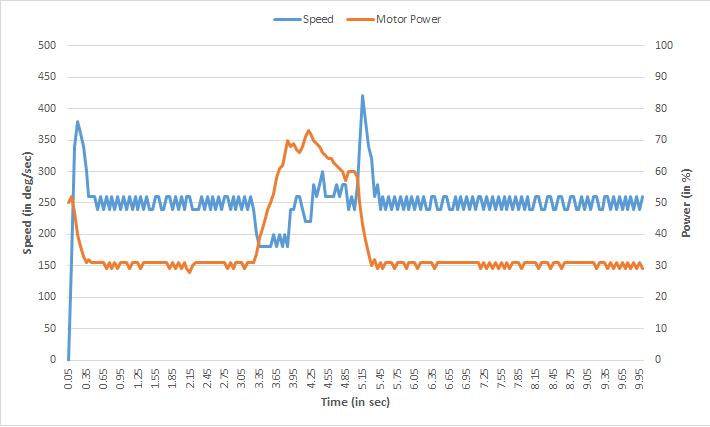
\includegraphics[width=0.5\textwidth]{PIDplot}
	\caption{Plot of Speed vs PWM level of the LEGO motor}
	\label{fig:PIDplot}
\end{figure}

As can be seen from the plot, there is a dip in the speed of the motor between $3$ and $5$ seconds which caused an increase in the PWM power level applied to the motor. When the friction is removed, the speed shoots up due to higher power level before settling down to the desired speed of $250$ deg/sec.

\subsection{Design and tuning of PID controller}
how to disable internal PID controller.
writing your own PID controller.
Zeigler-Nichols tuning
Critical damping

\subsection{System Identification using Bode plots}
brief on Bode plots
obtaining bode plots from experimental data
system identification using bode plots

\subsection{System Identification and Verification using MATLAB}
Introduction on System Identification.
brief on System identificaion Toolbox in MATLAB
Simulink model for identification and verification.

\section{Conclusions for Analysis of LEGO DC Motor}
summary of concepts learned through this set of experiments
comparison to current practices

\section{NXTway-GS - A two wheeled self-balancing robot}
The second half of the report details the building of a 2-wheel Self-balancing robot using the LEGO NXT kit and a HiTechnic Gyro Sensor. The 2-wheel Self-balancing robot can be modelled as a \emph{2D Inverted pendulum} system which is a well studied classic problem in Control Engineering. This makes it ideal for a 1 month course project in a first year Masters programme in Control Engineering. The analysis is divided into 3 parts - 1. Mathematical Modelling, 2. Servo PID Controller design and 3. Experimental Results. MATLAB provides official Simulink support package for LEGO Mindstorms NXT hardware which allows the students to use the various toolboxes available in Simulink and deploy the model to the LEGO NXT hardware.

\subsection{Modelling the 2-wheel Self-balancing Robot}
The 2-wheel Self-balancing Robot can be modelled as a 2-wheeled Inverted Pendulum system as shown in~Figure~\ref{fig:InvPen}. The mathematical model of such a system is derived here from first principles. 
\begin{figure}[!hbp]
	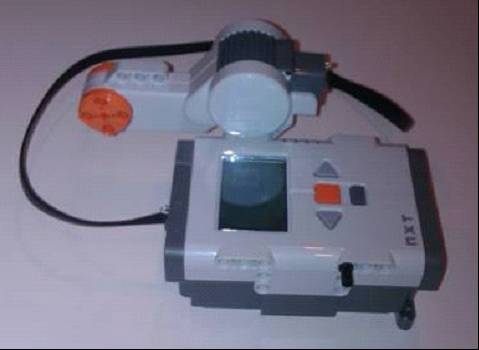
\includegraphics[width=0.5\textwidth]{InvPen}
	\caption{2-wheeled Inverted Pendulum}
	\label{fig:InvPen}
\end{figure}
The physical parameters used in the model with their nominal values have been tabulated in~Table~\ref{tbl:PhyPar} in Appendix B.

The equations of motion for the 2-wheeled inverted pendulum can be derived using the Lagrangian method based on the coordinate axis adopted in~Figure~\ref{fig:InvPen}. If direction of two-wheeled inverted pendulum is positive x-axis at $t=0$, then:

\begin{equation}
(\theta,\phi) = (\frac{\theta{}_{l}+\theta{}_{r}}{2},\frac{R(\theta{}_{r}-\theta{}_{l})}{W})
\end{equation}

\begin{tabular}{|l|l|l|}
\hline
Parameter & Nominal Value & Remark \\
\hline
$g$ & $9.81 m/sec^2$ & Accel. due to Gravity \\
\hline
$m$ & $0.03 kg$ & Wheel weight \\
\hline
$R$ & $0.04 m$ & Wheel radius \\
\hline
$J_{w}$ & $\frac{mR^2}{2} kgm$ & Wheel inertia moment \\
\hline
$M$ & $0.6 kg$ & Body weight \\
\hline
$W$ & $0.14 m$ & Body width \\
\hline
$D$ & $0.04 m$ & Body depth \\
\hline
$H$ & $0.144 m$ & Body height \\
\hline
$L$ & $\frac{H}{2} m$  & Dist. of CoM from wheel axle \\
\hline
$J_{\psi}$ & $\frac{ML^2}{3} kgm^2$ & Body pitch inertia moment \\
\hline
$J_{\phi}$ & $\frac{M(W^2+D^2)}{12} kgm^2$ & Body yaw inertia moment \\
\hline
$J_m$ & $1×10^−5 kgm^2$ & DC motor inertia moment \\
\hline
$R_m$ & $6.69 \Omega$ & DC motor resistance \\
\hline
$K_b$ & $0.468 Vsec/rad$ & DC motor back EMF constant \\
\hline
$K_t$ & $0.317 Nm/A$ & DC motor torque constant \\
\hline
$n$ & $1$ & Gear ratio \\
\hline
$f_m$ & $0.0022$ & Friction coeff. b/w body and DC motor \\
\hline
$f_W$ & $0$ & Friction coeff. b/w wheel and floor \\
\hline
\end{tabular}

\subsection{Controller Design}
Linearization about $\psi = 0$
State space representation 
Servo controller
Feedback gain calculations - LQR concepts
Integral gain to regulate steady state errors.

\subsection{Simulation and Verfication}
Simulation results
experimental results
graphs and diagrams

\subsection{Future work}
Possible extensions to the project

\section{Conclusions for two-wheeled self-balancing robot}
Summary of concepts learned through this project.
Time frame for the project.
Possible alterations

\section{Appendix}
\subsection{Zeigler-Nichols Tuning}
\begin{itemize}
\item Set Ki and Kd to zero.
\item Slowly increase Kp to a value Ku at which sustained oscillations - constant amplitude and periodic - are observed.
\item Note period of oscillation
\item Refer table below for initial values
\end{itemize}

\begin{tabular}{|l|l|l|l|}
\hline
       Z-N Model      & Kp       & Ki       & Kd       \\      
\hline
       P controller   & 0.5*Ku   & 0        & 0        \\
\hline
       PI controller  & 0.455*Ku & 0.833*Tu & 0        \\
\hline
       PID controller & 0.588*Ku & 0.5*Tu   & 0.125*Tu \\
\hline
\end{tabular}
\\
\\
Since Z-N method usually results in aggressive tuning, alternatively Tyreus-Luyben method can be adopted.
\\
\begin{tabular}{|l|l|l|l|}
\hline
       T-L Model      & Kp       & Ki     & Kd       \\
\hline
       PI controller  & 0.312*Ku & 2.2*Tu & 0        \\
\hline
       PID controller & 0.454*Ku & 2.2*Tu & 0.159*Tu \\
\hline
\end{tabular}
%%% End document
\end{document}